\documentclass[11pt]{article}
\textwidth 155mm \textheight 245mm \oddsidemargin -2mm
\evensidemargin -2mm \topmargin -20mm

\usepackage{graphicx}


\begin{document}

\begin{center}
  {\Large \bf A model of discrete random walk with
  history-dependent transition probabilities}

\medskip
    Petr Volf$^1$, Tom\'{a}\v{s} Kou\v{r}im$^2$,
 \smallskip\\
   {\small $^1$Institute of Information Theory and Automation, Academy of Sciences of the
  Czech Republic, Prague, {\em email: volf@utia.cas.cz}\\  
  $^2$Faculty of Nuclear Sciences and Physical Engineering,
  Czech Technical University in Prague, Czech Republic.}

\end{center}

\paragraph{Abstract.} This contribution deals with a model of
one-dimensional Bernoulli-like random
walk with the position of the walker controlled by varying transition
probabilities. These probabilities depend explicitly on the previous move
of the walker and, therefore, implicitly on the entire walk history. Hence, the walk is not Markov.
The paper follows on the recent work of the authors, the models present
here describe how the logits of transition probabilities are changing
in dependence on the last walk step. In the basic
model this development is controlled by parameters. In the more general setting
these parameters are allowed to be time-dependent, too.
The contribution focuses mainly on reliable estimation of model components
via the MLE procedures in the framework of the generalized linear models.

\paragraph{Keywords:} Bernoulli random walk, changing transition probabilities,
time dependent parameters, logistic model.

\section{Introduction}

The contribution presents a model of discrete time Bernoulli-like
random walk with probabilities of the next step depending on the
walk past. Namely, the steps of walk are $X_t=1$ or $0$, as a
variant the walk with steps $X_t =1, -1$ is considered.
Probabilities are $P_t=P(X_t=1)$, $t=1,2,...$, starting from
certain $P_1$. It is assumed that these probabilities develop and
depend on last walk steps making the walk a non-Markovian stochastic
process. A practical inspiration of such walk
type with steps 1, -1 comes from models of sport matches, for
instance of tennis, and sequence of its games, or in finer or
rougher setting, its balls or its sets. Similarly, walk with steps
1, 0 can model a series of events (e.g. failures, repairs) in a
reliability study, the ``step'' 1 denoting an event occurrence, ``step''
0 then means no event in time interval $t$. The later case in fact
corresponds to the discrete time recurrent events counting process
model, where both event occurrence and absence changes future event
probability. Thus, the models can be regarded as a simple discrete
variants of "self-exciting" point processes, cf. Hawkes (1971).

One set of studied random walk models, there with steps 1, -1, has
been proposed in Kou\v{r}im, Volf (2020), application to tennis
matches modelling and prediction was presented already in
Kou\v{r}im (2019). For illustration, let us here recall the
simplest form of such a model. Two parameters, the initial
probability $P_1$ and change parameter $\lambda$ are given, both
in $(0,1)$. The development of walk is described via the
development of the probability of step ``1'':
 $$
P_{t+1}=\lambda P_t+{1-\lambda\over 2}(1-X_t). \eqno{(1)}
 $$
In such a model, after event ``1'' its probability in the next step
is reduced by $\lambda$, therefore the model is called ``success
punishing''. A variant increasing $P_{t+1}$ after the occurrence of event ``1'', the
``success rewarding'' model, has
 $P_{t+1}=\lambda P_t+(1-\lambda) / 2 \cdot (1+X_t).$

In the paper of Kou\v{r}im, Volf (2020) several more complicated
model variants, with more parameters, were introduced and the
properties of models studied. Their limiting properties were
derived theoretically, while their behavior in small time horizon
was examined graphically, as it could be expected that in a
typical applied task the data would consist of a (sometimes quite
large) set of not too long walks. Again, examples include data from a number of sports matches or records on
reliability history of several technical devices during a limited
time period. Notice also that from a sequence having
$X_t=\pm 1$ a simple transformation $Y_t=(X_t+1)/2$ leads to a sequence
with values $Y_t=0,1$.

The models like (1) have an advantage that the impact of
parameters $\lambda$ to probability change is given rather
explicitly. Further, the proofs of large sample properties
(tendencies, limits) of walks as well as of the sequences of
probabilities are quite easy, at least in the simplest model
version, as shown in Kou\v{r}im, Volf (2020). On the other hand,
the computation of likelihood is complicated and the estimation of parameters
difficult. In fact, the estimation procedures should use random
search methods, approximate confidence intervals of parameters are
then obtained by an intensive use of random generator.

That is why the present paper introduces slightly different model
form, where instead the transition probabilities directly their
logits are changing. Thus, the model can be viewed as a case of
logistic model and solved by standard MLE approach, yielding
simultaneously asymptotic confidence intervals of parameters.
Therefore, we shall concentrate here to practical aspects of the
model, i.e. to aspects of model parameters estimation as well as
to model utilization. The question of easy and reliable estimation
will be even more important when we allow for time-dependent
parameters.

There exists a number of recent papers dealing
with discrete random walks and time series. The paper of
Davis and Liu (2016)  contains a rather
broad definition of such a process dynamics. Formally, our
definition is covered as well, however, certain basic assumptions, e.g.
the condition of contraction, are not fulfilled.

The monograph of Ch. Weiss (2018) offers a thorough overview of models  for discrete
valued time series, focusing also on discrete count data and categorical processes.
Models are accompanied by a number of real examples. The problem of process prediction and
the test of model fit is discussed as well,

The term ``self-excited'' discrete valued process is used quite frequently today,
however in a slightly different sense, see for instance Möller (2016) dealing with
discrete valued ARMA processes  and with their regime switching caused by the
process development (so called SETAR processes).

  \medskip
The rest of the paper is organized as follows: Next section
contains model formulation. Further, the method of the ML
estimation in the framework of logistic form of the general linear
models will be described and broadened to the case of
time-dependent model parameters. Then the properties of obtained
random sequences, not only of the process of observations but also
of the process of probability logits, will be discussed. Model
performance and its parameters estimation will be illustrated with
the aid of randomly generated examples. An example with
time-varying parameters will be included, too. Methods of both parametric and non-parametric
estimation of these functional parameters will be proposed and their performance checked.
Finally, a simple real data case, consisting of several series of recurrent events - failures and repairs,
will be presented. The solution is accompanied by a graphical method of testing the model fit.


\section{Model description}

Let transition probabilities be expressed in a logistic form,
namely $P_t=exp(a_t)/(exp(a_t)+1)$, i.e. $a_t=logit(P_t)$,
$t=1,2,...$, and let their development be described via the
following development of $a_t$,
starting from an initial $a_1$:\\
  1. In the case of steps $X_t= 1$ or 0:
   $$
a_{t+1}=a_t+c_1 X_t+c_2 (1-X_t)  = a_t+c_2+X_t (c_1-c_2).
\eqno{(2)}
  $$
 2. For the walk with steps $X_t= 1$ or -1:
    $$
a_{t+1}=a_t+c_1 (1+X_t)/2+c_2 (1-X_t)/2
  = a_t+(c_1+c_2)/2+X_t (c_1-c_2)/2.
 $$
Parameters $c_j,\,j=1,2$ as well as $a_1$ can attain all real
values (though values far from zero are not expected in real
cases), hence it is quite natural to test whether they are
significantly different from zero, or whether they are positive
(negative), whether $c_1=c_2$, etc. Notice also that $c_1<0$
reduces the probability of success $P_{t+1}=P(X_{t+1}=1)$ after
$X_t=1$, while the value of $c_2$ shows the reaction of
probabilities to the opposite result (0 or -1).

Further, it is observed that the model can be re-parametrized, in
case 1. using parameters $c_2$ and $d=c_1-c_2$, in case 2.
with $d_1=(c_1+c_2)/2,\,d_2=(c_1-c_2)/2$.

\section{Log-likelihood and the MLE}

{\bf 1. For the case $X_t=1,\, 0$ and $t=1,2,...,T:$}

 The likelihood function for one process of length $T$ equals
 $$
 {\cal L}=\prod_{t=1}^{T} P_t^{X_t}\cdot (1-P_t)^{(1-X_t)}
 =\prod_{t=1}^{T} \exp[a_t X_t]\cdot {1\over \exp(a_t) +1}.
 $$

Further, $a_{t+1}=a_t+c_2+X_t d = a_1+t c_2+d\sum_{j=1}^t X_j.$
Again, except for a given (and possibly unknown) starting $a_1$ all other
$a_t$ are random.

As a rule we observe $N$ processes, i.e. their outcomes $X_{t,i},
t=1,...,T,\,i=1,...N$. It is assumed that the parameters $a_1, c_1, c_2$
are common, however $a_t=a_{t,i}$ develop randomly for $t>1$. Then the
log-likelihood function equals
 $$
 L=\sum_{i=1}^N \sum_{t=1}^{T} \{ X_{t,i} a_{t,i}- \ln (\exp(a_{t,i})+1)\},
 $$
where  $a_{t+1,i}= a_1+t c_2+d \sum_{j=1}^t X_{j,i}.$
Continuing, with notation $Y_{t,i}=\sum_{j=1}^t X_{j,i}$, we get
 $$
L=\sum_{i=1}^N \{ a_1 \sum_{t=1}^T X_{t,i} + c_2 \sum_{t=1}^{T-1}
t X_{t+1,i}
 +d \sum_{t=1}^{T-1} X_{t+1,i} Y_{t,i}
 -\sum_{t=1}^{T} \ln (\exp(a_{t,i})+1)\}.
   \eqno{(3)}
 $$

\medskip
{\bf 2. For the case $X_t=1,\, -1$, $t=1,2,...,T:$}

Now, for one process
 $$
{\cal L}=\prod_{t=1}^{T} P_t^{(1+X_{t})/2}\cdot (1-P_t)^{(1-X_{t})/2}=
\prod_{t=1}^{T} \exp[a_t (1+X_{t})/2]\cdot {1\over \exp(a_t) +1},
$$
where $a_{t+1}= a_{t}+d_1+X_t d_2=a_1+d_1 t
+ d_2 \sum_{j=1}^t X_j.$
Hence, the full log-likelihood equals
$$
 L=\sum_{i=1}^N \sum_{t=1}^{T} \{ {1+ X_{t,i}\over 2} a_{t,i}
 - \ln (\exp(a_{t,i})+1)\}=
 $$
 $$
=\sum_{i=1}^N \{ a_1 \sum_{t=1}^T {1+ X_{t,i}\over 2} + d_1
\sum_{t=1}^{T-1} t {1+ X_{t+1,i}\over 2}
 +d_2 \sum_{t=1}^{T-1}{1+ X_{t+1,i}\over 2} Y_{t,i}
 -\sum_{t=1}^{T} \ln (\exp(a_{t,i})+1)\},
   \eqno{(4)}
 $$
where again $Y_{t,i}=\sum_{j=1}^t X_{j,i}$.

\medskip
In both variants the model can be treated in the framework of
logistic regression model. Then, both the 1-st and 2-nd
derivatives of $L$ are tractable and the MLE as well as the
asymptotic variance of estimates can be computed with the aid of
a convenient numerical procedure (e.g. the Newton--Raphson
algorithm). In fact, these algorithms are included standardly in
data-analysis software packages, mostly as a part of methods for
generalized linear models. Numerical examples presented here will
utilize the Matlab function {\it glmfit.m}.

In the sequel we shall deal just with the first model type
considering the random walk with steps 1 or 0.

\section{On properties of sequences $a_t$ and $P_t$}

In Kou\v{r}im and Volf (2020) some interesting properties of model
(1) have been derived. It focused on the development of the random
sequences of probabilities $P_t$ as well as of sums
$S(t)=\sum_{s=1}^t X_s$. Now, we shall discuss the behavior of
random sequences of $P_t$ and their logits $a_t$ of model (2). Let
us summarize here some of its basic properties:

 \begin{description}
\item i) It is seen that $a_{t+1}=a_1+k_1\cdot c_1 + k_2\cdot
c_2$, where $k_1, k_2$ are (random) nonnegative integers,
$k_1+k_2=t$. Hence, the domain of values $a_t$ is discrete and
finite, being larger and larger when time grows.

\item ii) $a_t$ is a Markov sequence, as $a_{t+1}=a_t+c_1$ with
probability $P_t$ determined by $a_t$, or $a_{t+1}=a_t+c_2$ with
probability $1-P_t$. Hence, transition from state $a$ depends
just on this state. This Markov chain is thus homogeneous, as long
as parameters $c_j$ are constant.

On the other side, the sequences $X_t$ and $S_t$ are not Markov, while the
bi-variate processes $(X_t, a_t)$ and $(S_t, a_t)$ have the Markov property.

\item iii) Further, from i) it follows that the return of $a_t$ to
some of previous values could be impossible (for instance in the
case of irrational $c_1, c_2,\, c_1\ne -c_2$). When the return is
possible, its period is at least 2; this case occurs when
$c_1=-c_2$. Hence, in general, the chain cannot have any
stationary distribution.

\item iv) From i) it also follows that when both $c_1, c_2$ are
positive (negative), $a_t \to \, +\infty\,\,(-\infty)$ a.s.
Hence, the only interesting could be the case when $c_1, c_2$ have
different signs.
 \end{description}

\subsection{A model with one parameter}

Let us mention here also a special case with unique parameter
$c=c_1=-c_2$. Then $a_{t+1}=a_1+k\cdot c,$ $k$ is a random, integer from
$[-t, t]$. When $c<0$, then the sequence reduces the probability
of repetition of preceding result, the model is then a variant of the
``success punishing'' model (1). The opposite case occurs when
$c>0$. In Kou\v{r}im and Volf (2020) dealing with model (1),
certain closed formulas for limit of expectations and variances
E$(P_t)$, Var$(P_t)$ were derived. Though now the limit behavior
seems to be quite similar, we are not able to describe it
precisely. On the other hand, it is easy to compute transition matrices
and then to follow the development of distributions of both $a_t$ and $P_t$
 for given $c$ and initial $a_1$.

\begin{figure}[h]
\centering
    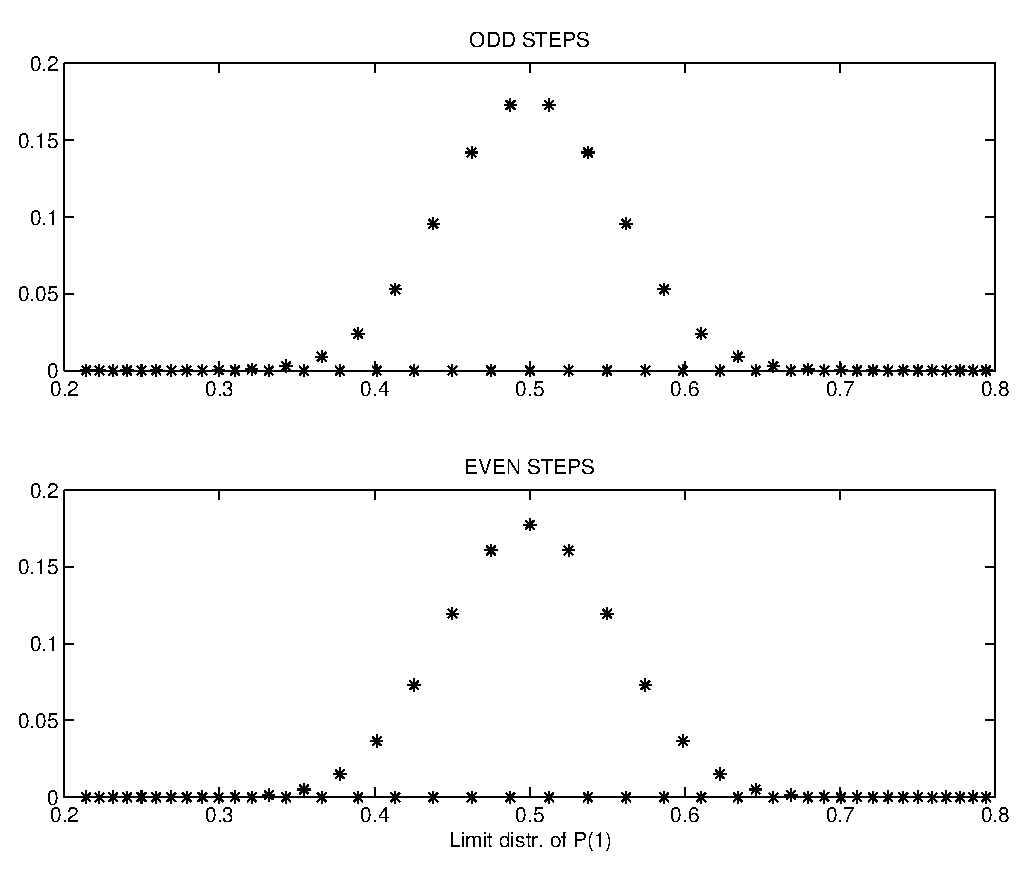
\includegraphics[width = 10cm,height=7cm]{vyvoj_s_punish.eps}
\caption{Approximate limit distribution of $P_t$ when $a_1=0.2,\,
c=-0.05$.}
\end{figure}

\subsubsection{Case with $c<0$}

Figure 1 shows an approximation of limit distributions of $P_t =P(X_t=1)$ when $t\to\infty$, separately for 
even and odd $t$, in the case $a_1=0.2,\, c=-0.05$. More precisely, the figure shows the distribution of $P_t$ after
400 and 401 steps, respectively. In both cases, final E$P_t$=0.500002, Var$P_t$=0.003087, the change of distributions in the last 2 steps was already smaller than $10^{-7}$.

Thus, the figure indicates that both stationary distributions are centered around 0.5 
(hence, corresponding limit distribution of $a_t$ around zero). Further, 
it was revealed that the limit distribution does not depend on
initial $a_1$, however it depends on $c$: though the mean still tends to 0.5,
the limit variance is smaller for $c$ closer to zero.

\begin{figure}[h]
\centering
    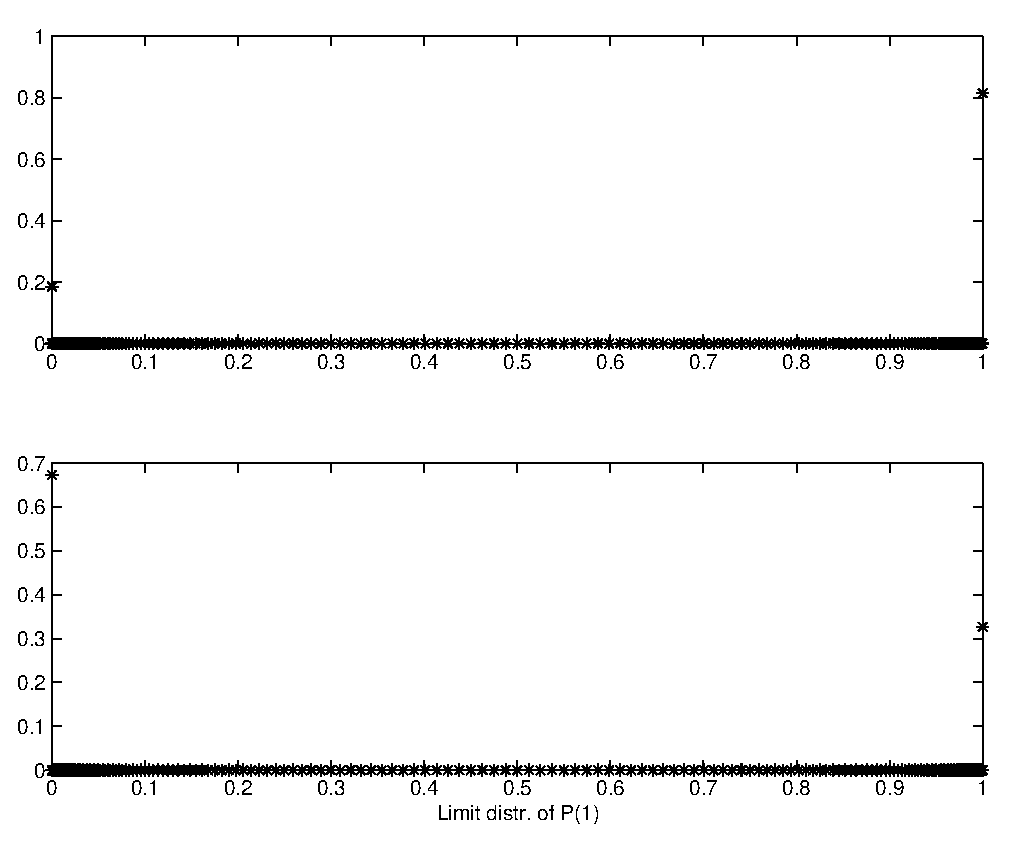
\includegraphics[width = 10cm,height=7cm]{vyvoj_s_reward.eps}
\caption{Approximate limit distribution of $P_t$: Above for
$a_1=0.2,\, c=0.05$, below for $a_1=-0.1,\, c=0.05$.}
\end{figure}

\subsubsection{Case with $c>0$}

Figure 2 shows the limit behavior of distribution of $P_t$ in the case of positive parameter $c$. 
It is seen that now the picture is quite different, the figure indicates that the limit distribution is
``unproper'', equal to a Bernoulli distribution with certain $\cal{P}$ such that $Prob(P_t\to 1)=\cal{P}$, while $Prob(P_t\to 0)=1-\cal{P}$.
Notice that it corresponds to $a_t$ tending to $\pm \infty$, with the same probabilities.
Moreover, it was revealed that $\cal{P}$ depends on both $a_1$ and $c$.
The upper subplot of Figure 2 shows the distribution of $P_t$ in 
the process starting from $a_1=0.2$ and with $c=0.05$, after 1000 steps 
(the limit behavior of the sequence with odd and even steps is comparable).
In fact, as it is possible to work computationally just with finite matrices and domains of values, we set values
$a=a_1\pm 300\cdot c$ as absorbing states. Regarding the domain of $P_t$, absorbing states were then
$Pmin\approx 4\cdot 10^{-7},\, Pmax\approx 1-3\cdot 10^{-7}$. Final distribution had
E$P_t = 0.814653$ (in fact it is the estimate of probability $\cal{P}$), Var$P_t=0.1508043$, while E$P_t\cdot (1-$E$P_t)=0.1508045$
(this could be taken as an indication how close we are already to Bernoulli distribution).

The lower subplot of Figure 2 shows the same for the case with $a_1=-0.1,\,c=0.05$.
Now, after 1000 steps and with absorbing states constructed as above, we obtained
E$P_t = 0.327023$, Var$P_t=0.2200786$, while E$P_t\cdot (1-$E$P_t)=0.2200789$.

%%%%%%%%%%%%

\section{Time dependent parameters}

In many instances the impact of walk history
to its future steps could be changing during observation period and
therefore the time-dependent parameters $c_1=c_1(t),\,c_2=c_2(t)$
should be considered. Then $d=c_1-c_2=d(t)$ as well. It opens a
question of their flexible estimation. The problem is solved quite
similarly as in other regression model cases: Either the
parameters-functions are approximated by certain functional types
(polynomial, combination of basic functions, regression splines)
or constructed by a smoothing method, similar to moving window or
kernel regression approach. The method described in Murphy and Sen
(1991) is of such a type and  concerns the Cox regression model. All these approaches can again be
incorporated to the logistic model form, just the number of
parameters will be larger. For instance, in the following examples
we shall use cubic polynomials for both estimated ``parameters''
$c_2,\, d$ (hence $c_1=c_2+d$ will also be a cubic polynomial),
each will be given by four parameters of cubic curve.

Further, in the last example the non-parametric moving window ML method was used as well.
Namely, while $a_1$ was kept constant, both $c_2(t)$ and $d(t)$ were estimated repeatedly
with the aid of Gauss kernel centered  at a set of points $T(1),...,T(M)$ selected among 1,....M-1.
These rough estimates then were smoothed secondary, again with a Gauss kernel. Then, the final
ML estimate of $a_1$ with $c_2(t),\ d(t)$ already fixed, was computed.

Another often used method dealing with time-dependent parameters
is based on the Bayes approach, it treats each such time-evolving
parameter as a random dynamic sequence with a prior model of its
development (Gamerman, West, 1986).

\section{Numerical examples}

The objective is, firstly, to study the behavior of processes, and,
secondly, to examine how well the MLE performs in the case of
constant parameters as well as in the case when they are
time-evolving.

\subsection{Artificial data}

In the first example the data were generated from the model with
initial $a_1=0.3$ and constant parameters $c_1=-0.7,\,c_2=0.5$.
Two cases were compared, in the first one just 20 walks of length
20 steps were generated. The MLE yielded the following estimates
(their standard errors based on approximate normality of the MLE are in
parentheses):

$a_1=0.3996 (0.2133),\,c_2=0.5869 (0.0887),\, d=-1.4802 (0.2017)$,

hence $c_1=c_2+d= -0.8214 (0.1116).$

It is seen that even for this case with small number of
observations the estimates are quite reasonable, except that the
standard error for $a_1$ is rather large (P-value of the test of
nullity of $a_1$ equals 0.0610).

In the second attempt with the same model, 100 walks, each with
100 steps, were generated. Now the results of the MLE are much
more precise:

$a_1=0.3007 (0.0454),\,c_2=0.5057 (0.0151),\, d=-1.2173 (0.0362)$,

 $c_1=c_2+d= -0.7099 (0.0211).$

Figure 3 then shows the development of $a_t$ and $P_t$, namely their
averages and variances from generated 100 walks. It is seen that
both stabilize rather quickly, as a consequence of negative $c_1$
and positive $c_2$ reducing $P_{t+1}$ after event $X_t=1$ and
increasing it after $X_t=0$.

\begin{figure}[h]
\centering
    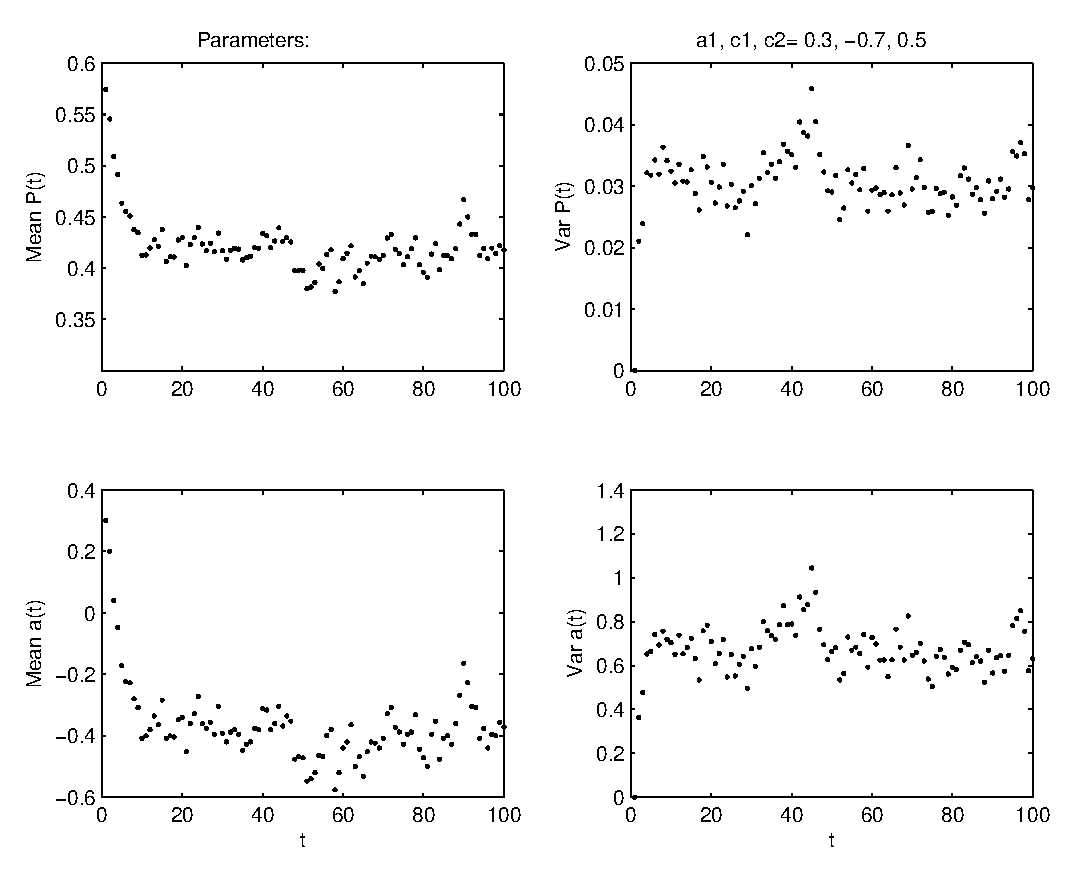
\includegraphics[width = 12cm,height=8cm]{simgener1.eps}
\caption{Sample means and variances of $a_t$ and $P_t$.}
\end{figure}

\begin{figure}[h]
\centering
    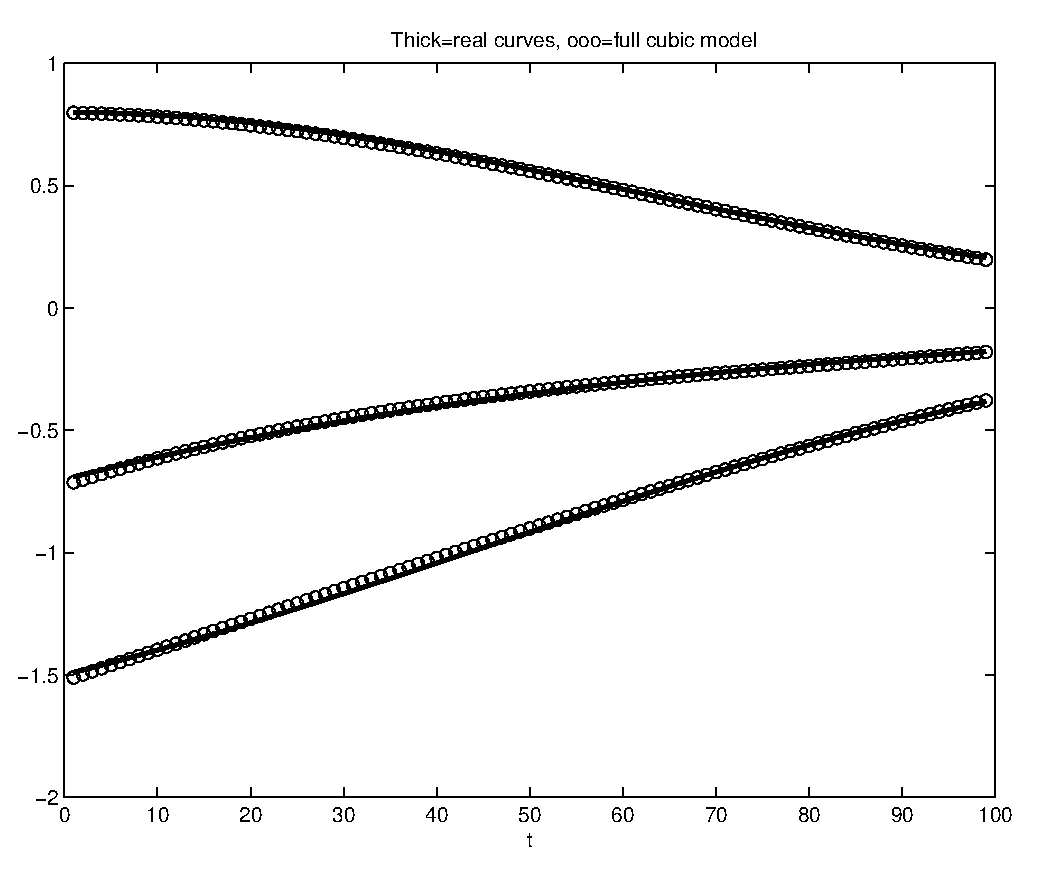
\includegraphics[width = 10cm,height=5cm]{simest_t.eps}
 \caption{Functional parameters (thick lines, from above
$c_2(t), c_1(t), d(t)= c_1(t)-c_2(t)$) and their estimates with
complete cubic functions (circles).}
%\end{figure}

%\begin{figure}[h]
\centering
   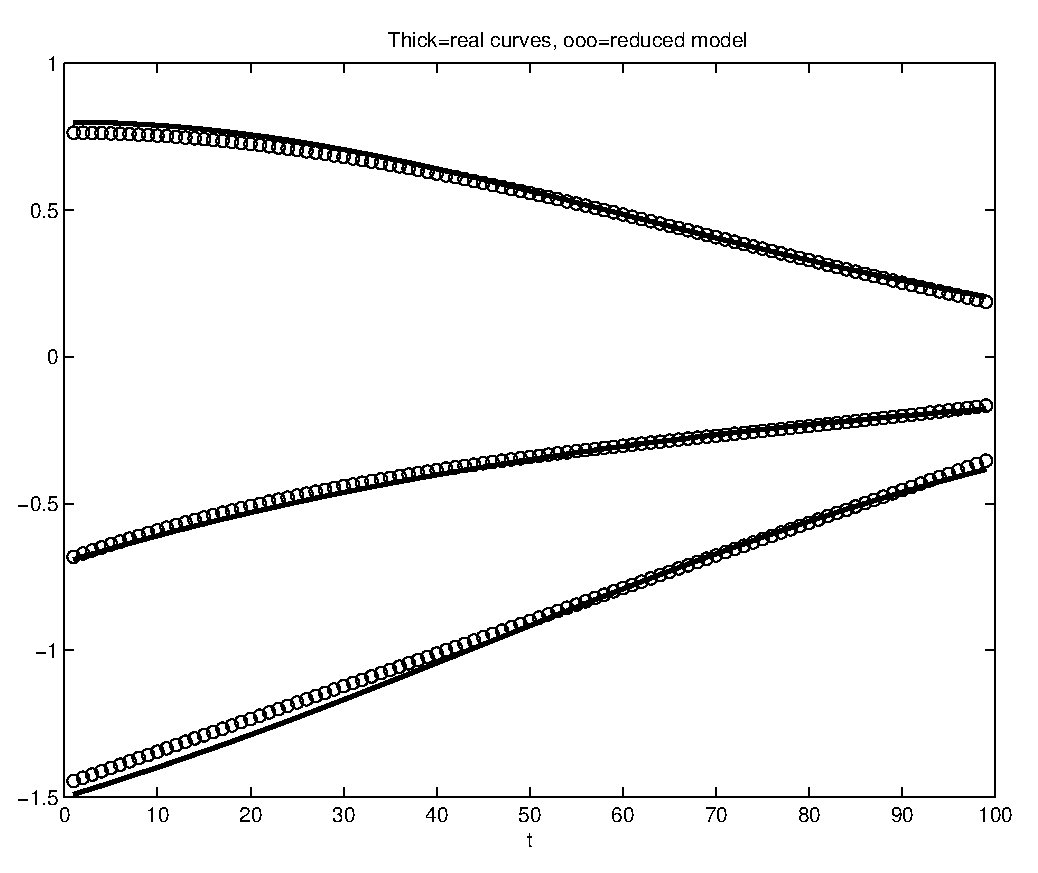
\includegraphics[width = 10cm,height=5cm]{simest_t_reduced.eps}
\caption{Functional parameters (thick) and their estimates via
reduced cubic model (circles).}
\end{figure}

\section{Parameters as functions of time}

In the next simulated example functional ``parameters'' were
considered. Namely, walks had again length 100 steps, $a_1=-0.2$,
the first $c_1(t)=-0.7\cdot (0.25)^{(t/100)}$ was increasing
exponential curve, the second $c_2(t)=0.8\cdot (0.25)^{(t/100)^2}$
was decreasing S-curve. Again, 100 such walks were generated.
Functions $c_1(t)$ and $d(t)=c_1(t)-c_2(t)$ were estimated as
cubic polynomials, in the logistic model framework. Results,
a sufficiently good approximation to real curves, are seen from
Figure 4. Initial $a_1$ was estimated as -0.1464, with P-value of
its nullity test 0.1468 (hence, its nullity cannot be rejected).
These results, however, correspond to the full model, some
parameters of both cubic curves were not significant, therefore a
sequential reduction of the model was performed. Namely, at each
reduction step one of the components with non-significant
parameters (i.e. the one with the largest p-value of the test
based on the MLE asymptotic normality) was removed from the model.
Thus, the final model, with all components significant, had
functions $c_2(t)=\alpha_0+\alpha_2 t^2+\alpha_3 t^3$ and
$d(t)=\beta_0+\beta_1 t$. The values of estimates were
$a_1=-0.1553$ (p-value=0.0283), further $\alpha_0=0,7640,
\alpha_2= -0,00011, \alpha_3=4,8e-07, \beta_0=-1,4560,
\beta_1=0,0111$, all corresponding p-values were already quite
negligible. Figure 5 shows the results of this last model.


\begin{figure}[h]
\centering
    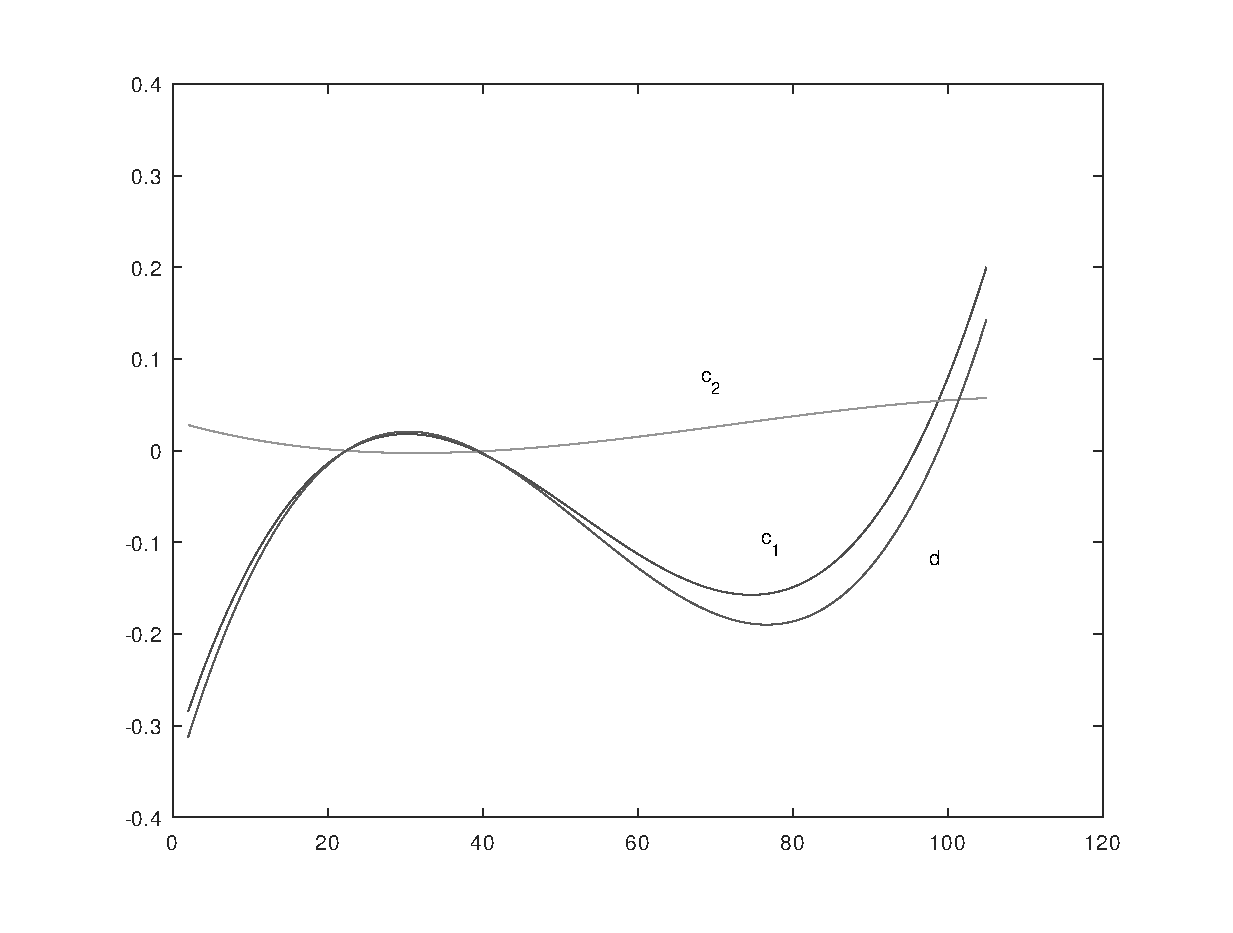
\includegraphics[width = 11cm,height=5cm]{comp_polyn.eps}
% \caption{.}
%\end{figure}

%\begin{figure}[h]
\centering
   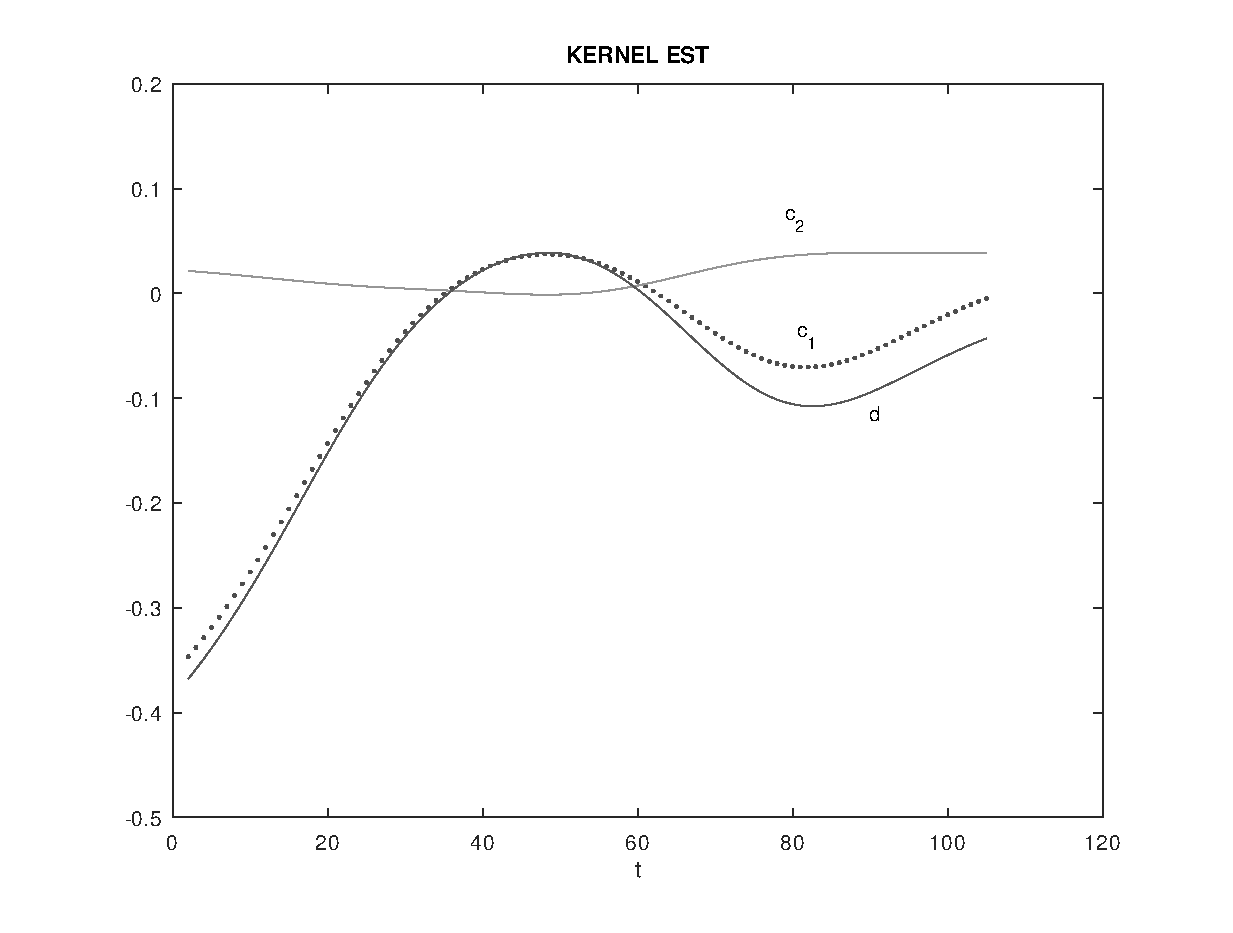
\includegraphics[width = 11cm,height=5cm]{comp_kern.eps}
\caption{Estimates of model functions. Above: cubic model, below: mowing window estimates.}
\end{figure}

\subsection{Real data case}

The following data are taken from Exercise 16.1 of Meeker, Escobar
(1998). The data are records of problems (failures, troubles) with
10 computers, each followed for 105 days. The table displays
the computer number and then days of reported and repaired
troubles.

\medskip

   401: 18, 22, 45, 52, 74, 76, 91, 98, 100, 103.

   402: 11, 17, 19, 26, 27, 38, 47, 48, 53, 86, 88.

   403: 2, 9, 18, 43, 69, 79, 87, 87, 95, 103, 105.

   404: 3, 23, 47, 61, 80, 90.

   501: 19, 43, 51, 62, 72, 73, 91, 93, 104, 104, 105.

   502: 7, 36, 40, 51, 64, 70, 73, 88, 93, 99, 100, 102.

   503: 28, 40, 82, 85, 89, 89, 95, 97, 104.

   504: 4, 20, 31, 45, 55, 68, 69, 99, 101, 104.

   601: 7, 34, 34, 79, 82, 85, 101.

   602: 9, 47, 78, 84.

\medskip

Thus, from our point of view, 10 walks, each of length 105 time
units, were observed. Steps $X_t=1$, representing the events = reported
troubles, were rather sparse, just 91, in the rest of days
$X_t=0$, i.e. nothing has occurred. Nevertheless, it could be
expected that the wear of devices was increasing.

First, the model with constant parameters was fitted. The results
were the following (again with asymptotic standard deviations in
parentheses):

$ a_1=-3.0368 (0.2578),\,c_2=0.0122 (0.0062),\, d=-0.0145
(0.0640)$,
hence $c_1 =  c_2 + d = -0.0022 (0.0592)$.

It is seen that $c_1<0$, though non-significantly, which means
that after a failure and repair the probability of further failure
decreased slightly. On the other hand, positive $c_2$ means that
the probability of failure increases in time, linearly in the
framework of model with constant parameters. Achieved maximal log-likelihood value
equaled -295.54.

In the next attempt, the model allowing cubic dependence of
both $c_1(t),\,c_2(t)$ on time was applied. Its maximum likelihood
estimate was obtained, however the most of the parameters were not
statistically significant, i.e. they were close to zero and
corresponding normal tests of their nullity had large p-values.
Again, the model was then reduced sequentially, at each step the
parameter with the largest (and larger than 0.1) p-value was
eliminated. Quite astonishingly, this procedure lead to a rather
plain model with $c_2(t)=\beta\cdot t^2$ and function $d(t)$
omitted, namely $a_1=-2.7797,\, \beta= 3.2931e-06$, corresponding
p-values were $3e-63,\,0.0003$. It means that in fact
$c_1(t)=c_2(t),$ an interpretation is that the influence of events
$X_t=1$ is rather negligible and the probability of such events is
increasing (slightly, but significantly) in time. In fact, its
logit $a(t)$ increases cubically, as from expression (2) we have
now that $a_{t+1}=a_1+\beta\sum_{s=1}^t s^2$. On the other side,
while the maximum likelihood corresponding to the full cubic
model was -292.49, the value achieved by the reduced model was
slightly smaller, -293.86.

Finally, the moving window method was utilized, too. Figure 6
shows both the full cubic model in its upper subplot and the
mowing window estimates, in lower subplot. It is seen that they
are quite comparable. Final estimate of parameter $ a_1 =
-2.7189$, the maximum of log-likelihood was -293.42.
 It is seen that the results of all these models, including the model
with constant parameters, were quite comparable in terms
of maximal log-likelihood. On the other side,
certain differences of their fit can
be traced from the following graphical analysis.


\subsection{Graphical test of model fit}

In general, the objective of goodness-of-fit tests is to decide
whether the model corresponds to observed data. There are several
possibilities, consisting mostly of the comparison of certain
characteristics of observed data with the same characteristics
derived from the model. We decided to consider, as the
characteristics suitable for graphical comparison, the cumulated
processes of steps of all walks together. In our case it equals
${\cal N}(t)=\sum_{i=1}^N \sum_{s\le t} X_i(s)$, which is in fact
the process counting observed events, the discrete-time counting
process.

A good model should be able to generate comparable sequences of
events. Therefore, when new walks (the same number and length) are
generated from the model, their aggregated counting process should
be similar to process observed. When such a generation is done
many times, a ``cloud'' of counting processes is obtained. In the
graphical test form, this cloud of processes generated from the
model should be around the process obtained from data. It is
illustrated on the next Figure 7. All three models presented above
were compared with real data. It is seen that the constant model
(upper plot) underestimates (from the beginning) and overestimates
(for larger times) the real process development. The other two
models perform better, the full cubic model's fit (middle plot) does
not seem to be worse than the non-parametric model in the lower
plot.

\begin{figure}[h]
\centering
    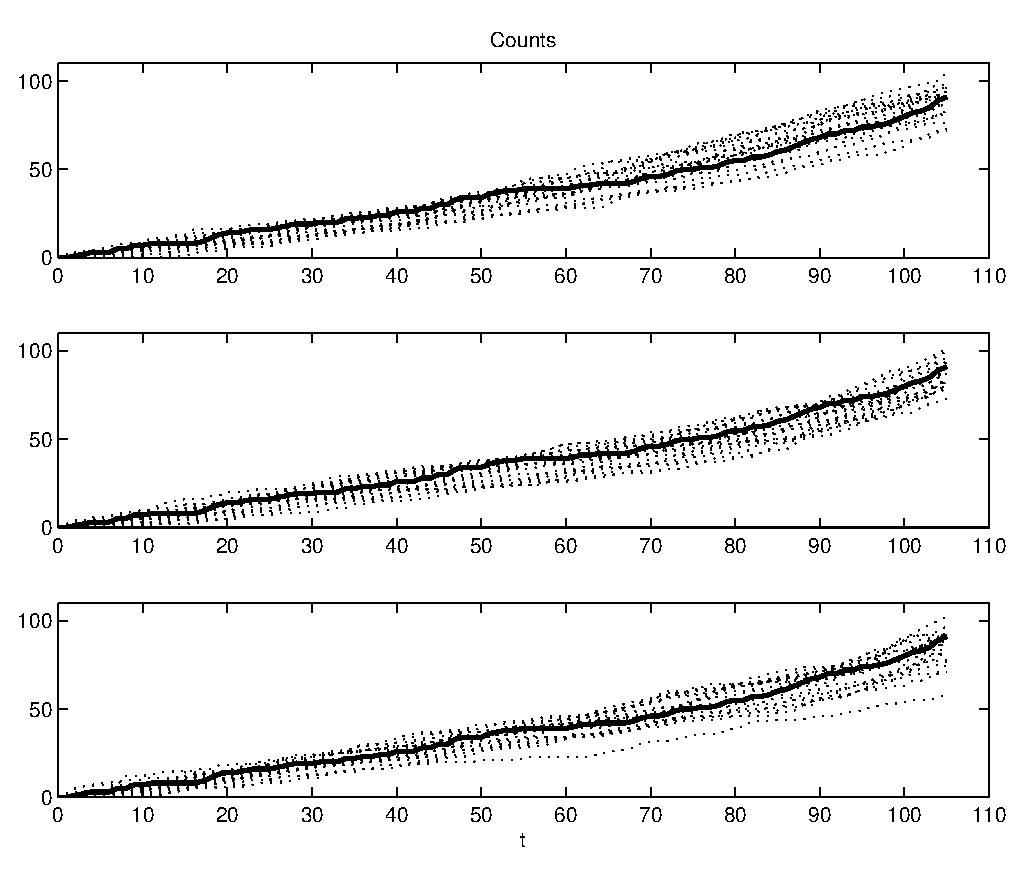
\includegraphics[width = 12cm,height=10cm]{comp_fit.eps}
\caption{Thick curve = real observed counting process of failures.
Clouds of dotted curves = counting processes generated from
estimated models. Top: constant model, middle plot: full cubic
model, bottom: model from mowing window estimates.}
\end{figure}

\section{Concluding remarks}

Standard non-parametric estimator in the count data setting is the
Nelson-Aalen estimator of the cumulative hazard function. In the
case of our real data example it is given by observed counting
process $\cal{N}(t)$ divided by the number of objects, as all objects
are ``at risk'' during the whole observation period. However, such
an estimator does not take into account possible dependence of
future risk on objects history. It could be incorporated via a
regression model modeling the hazard rate change after occurred
event. Hence, hazard function is in fact a random function.

Models proposed in the present paper offer an explicit description
of such an impact of process history to actual count
probabilities. A generalization may consist of considering a
longer memory, we have explored just models with memory 1.
Further generalization could include an influence of covariates to
probability logits.
The model's form makes it easy to model using logistic regression.
On the other hand, from this point of view
certain observable events from the process history could be taken as covariates, too.
In models studied here, this role is played by the last preceding process value.

Statistical analysis of processes of recurrent events has,
moreover, to take into account possible heterogeneity of studied
objects, in particular when dealing with medical, demographic or
also with economic data (see e.g. Winkelmann, 2008, Ch. 4). In such
a case, an additional random effect variable (called also the
frailty variable) should be added to the logit model. Procedure of
estimation then uses an alternation of two steps estimating
frailty values and the rest of model, respectively. Thus, the concept of heterogeneity
offers another way how the models studied in the present paper could be enriched.

\paragraph{Acknowledgement.}
The research was supported by the grant No. 18-02739S of the Grant
Agency of the Czech Republic.

\begin{thebibliography}{99}

\bibitem{dl} Davis, R.A., Liu, H.: Theory and inference for a class
of observation-driven models with application to time series of
counts. Statistica Sinica, 26 (2016), 1673-1707.

\bibitem{gw} Gamerman, D., West, M.: An
application of dynamic survival models in unemployment studies.
The Statistician, 36 (1987),  269-274

\bibitem{ha} Hawkes, A.G.: Spectra of some self-exciting
and mutually exciting point processes. Biometrika, 1971, 89-90.

\bibitem{ko} Kou\v{r}im, T.: Random walks with memory applied to
grand slam tennis matches modeling. In Proceedings of MathSport
International 2019 Conference (e-book). Propobos
Publications (2019)  220-227.

\bibitem{kovo} Kou\v{r}im, T., Volf, P.: Discrete random processes with memory:
Models and applications. Applications of Mathematics, 65, 3
(2020), 271-286.

\bibitem{me} Meeker, W.Q, Escobar, L.A.: Statistical methods for reliability
data. Wiley, 1998.

\bibitem{mo} Möller, T.A.: Self-exciting threshold models for time series
of counts with a finite range. Stoch. Model., 32 (2016), 77-98.

\bibitem{ms} Murphy, S.A., Sen, P.K.: Time-dependent coefficients
in a Cox-type regression model. Stoch.Proc. and
Applications, 39 (1991), 153-180.

\bibitem{we} Weiss, Ch.H.: An Introduction to Discrete Valued Time Series.
Wiley,  2018.

\bibitem{wi} Winkelmann, R.: Econometric Analysis of Count Data. Springer,  2008.

\end{thebibliography}

  \end{document}
